% ECE 506 project report: local and board2 experiments completed 2026-11-18.
% Compile from this directory with a PDF-capable LaTeX engine when desired.
% This delivery contains TeX source only; no report PDF has been generated.
\documentclass[11pt,letterpaper]{article}
\usepackage[margin=1in]{geometry}
\usepackage[T1]{fontenc}
\usepackage{lmodern}
\usepackage{microtype}
\usepackage{amsmath,amssymb}
\usepackage{booktabs,array}
\usepackage{graphicx}
\usepackage{tikz}
\usetikzlibrary{arrows.meta,positioning,fit}
\usepackage[hidelinks]{hyperref}
\graphicspath{{../figures/}{figures/}}
\setlength{\parindent}{0pt}
\setlength{\parskip}{0.5em}
\newcommand{\code}[1]{\texttt{\detokenize{#1}}}
\title{HLS Optimization of a Two-Layer FFN:\\Compute Parallelism and Weight-Memory Organization}
\author{Yuxin Ren \and Dongwei Wang}
\date{ECE 506: Reconfigurable Computing --- Fall 2026\\Experimental results, November 18, 2026}

\begin{document}
\maketitle

\begin{abstract}
This project studies how compute parallelism and on-chip weight delivery jointly
affect a fixed-point FPGA accelerator. We implement a $64\rightarrow128\rightarrow64$
feed-forward network (FFN) with runtime-loaded parameters and evaluate twelve HLS
configurations on the XC7Z020 at a common 100\,MHz target. All configurations pass
206 deterministic reference comparisons; four representative configurations also
pass RTL co-simulation. Increasing both output and input parallelism to four
reduces the HLS computation estimate from 18,181 to 1,669 cycles when the weight
memory supplies sufficient operands. The same arithmetic parallelism with
unpartitioned single-port weight memories requires 17,029 cycles and achieves an
initiation interval of 16. Packing four weights per word preserves the 1,669-cycle
estimate while reducing total estimated BRAM usage from 36 to 20 BRAM\_18K units.
The pipelined scalar baseline and packed design both complete placement and
routing at 100\,MHz. Additional reset and AXI tests pass for both deployment
candidates. On a physical PYNQ-Z2, both selected designs pass all 206
correctness cases and 3,000 measured inference calls. The packed design reduces
Python/FPGA end-to-end median latency from 1.104 to 0.965\,ms, a $1.14\times$
improvement, while compiled board-CPU computation takes approximately
0.143\,ms. Thus the core optimization is effective, but host interaction and
buffer synchronization dominate the tested single-input system interface.
\end{abstract}

\section{Introduction and Related Work}
A dense matrix--vector product exposes parallelism across output neurons and
across the terms of each dot product. Unrolling these operations creates demand
for concurrent weight reads. Additional multipliers are therefore useful only
when the memory organization and accumulation schedule can supply them. Memory
partitioning can increase bandwidth, but its physical cost depends on the width,
depth, and number of the resulting banks.

Cilardo and Gallo analyze the interaction between loop unrolling and
multidimensional memory partitioning, including the area overhead associated
with partitioning~\cite{cilardo2015}. Their work motivates measuring the cost of
operand delivery alongside the number of arithmetic lanes. FINN-R explores
customized quantized neural-network inference engines and their performance and
resource trade-offs~\cite{blott2018}. Its separation of neuron-level and
input-level parallelism motivates the two parameters used here. Our study is a
controlled experiment on a small fixed-size FFN, rather than a reproduction of
either framework or its application benchmarks.

The experiments address three questions: how latency and resource usage change
with parallelism; how limited weight ports restrict unrolling; and whether wider
packed memories reduce the cost of supplying the same parallel arithmetic. The
workload, arithmetic, layer-level architecture, tool version, and clock constraint
remain common across the comparisons.

The contributions are a bit-exact, runtime-parameterized HLS implementation; a
twelve-configuration experiment that separates arithmetic parallelism from
weight-memory organization; and an implemented, board-validated comparison
against both the scalar FPGA baseline and compiled CPU execution. The board
experiment also tests whether a large computation-cycle improvement survives
the software and memory-system costs of single-input inference.

\section{Workload and Numerical Contract}
The network computes
\begin{align}
 h &= \mathcal{Q}_{16}\!\left(\operatorname{ReLU}(W_1x+b_1)\right),\\
 z &= \mathcal{Q}_{16}\!\left(W_2h+b_2\right),
\end{align}
where $x,z\in\mathbb{R}^{64}$, $h\in\mathbb{R}^{128}$,
$W_1\in\mathbb{R}^{128\times64}$, and
$W_2\in\mathbb{R}^{64\times128}$. Each invocation processes one input vector.
The two layers contain 16,384 multiply--accumulate terms in total. Deterministic
synthetic parameters and inputs make this an operator benchmark; no training,
classification accuracy, or application-quality claim is made.

Weights, activations, and biases are signed 16-bit integers representing
$\mathrm{raw}/1024$. Products have 20 fractional bits. For a single neuron, the
integer accumulator is
\begin{equation}
 A = 1024\,b_{\rm raw}+\sum_j w_{{\rm raw},j}x_{{\rm raw},j}.
\end{equation}
The HLS implementation uses signed 32-bit products and a signed 40-bit
accumulator; the independent C++ reference uses \code{int64_t}. Even a
128-term full-range dot product plus bias has magnitude less than $2^{38}$,
so 40 bits are sufficient. There is no truncation or saturation inside the dot
product. In the first layer, negative $A$ is clamped to zero before quantization.
At either layer boundary, rounding is to the nearest integer with ties away
from zero:
\begin{equation}
 r(A)=\begin{cases}
 \left\lfloor(A+512)/1024\right\rfloor,& A\geq0,\\
 -\left\lfloor(-A+512)/1024\right\rfloor,& A<0,
 \end{cases}
 \qquad
 \mathcal{Q}_{16}(A)=\min(32767,\max(-32768,r(A))).
\end{equation}
This common contract makes different accumulation groupings bit-exact.

The two weight matrices occupy 32\,KiB. Including 192 biases, a parameter set
contains 16,576 signed 16-bit values, or 33,152 bytes. The external layout is
row-major $W_1,b_1,W_2,b_2$, with four consecutive values packed into each
little-endian 64-bit word. Inputs and outputs each occupy 128 bytes. All designs
consume the same parameter and input files.

\section{Accelerator Architecture}
Figure~\ref{fig:architecture} separates the control, DDR transfer, and on-chip
computation paths. Parameters are transferred during LOAD and reused during RUN.

\begin{figure}[tb]
\centering
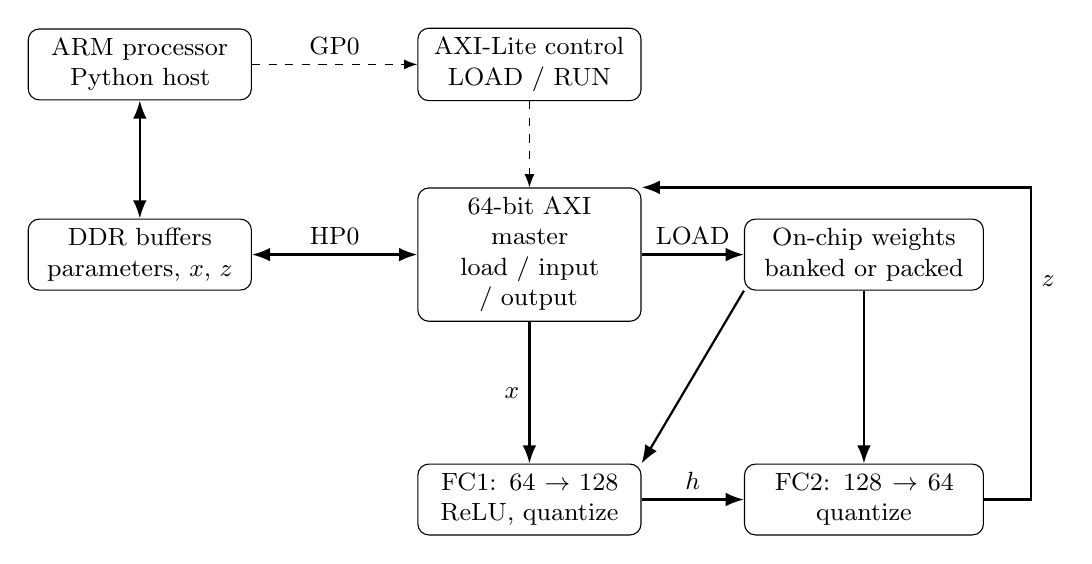
\begin{tikzpicture}[font=\small, >=Latex,
 box/.style={draw,rounded corners,align=center,minimum height=9mm},
 data/.style={->,thick}, control/.style={->,dashed}]
 \node[box,text width=26mm] (cpu) {ARM processor\\Python host};
 \node[box,text width=26mm,right=21mm of cpu] (ctrl) {AXI-Lite control\\LOAD / RUN};
 \node[box,text width=26mm,below=15mm of cpu] (ddr) {DDR buffers\\parameters, $x$, $z$};
 \node[box,text width=26mm,right=21mm of ddr] (io) {64-bit AXI master\\load / input / output};
 \node[box,text width=28mm,right=13mm of io] (weights) {On-chip weights\\banked or packed};
 \node[box,text width=26mm,below=18mm of io] (fc1) {FC1: $64\to128$\\ReLU, quantize};
 \node[box,text width=28mm,right=13mm of fc1] (fc2) {FC2: $128\to64$\\quantize};
 \draw[control] (cpu) -- node[above]{GP0} (ctrl);
 \draw[control] (ctrl) -- (io);
 \draw[<->,thick] (cpu) -- (ddr);
 \draw[<->,thick] (ddr) -- node[above]{HP0} (io);
 \draw[data] (io) -- node[above]{LOAD} (weights);
 \draw[data] (io) -- node[left]{$x$} (fc1);
 \draw[data] (weights) -- (fc2);
 \draw[data] (weights.south west) -- (fc1.north east);
 \draw[data] (fc1) -- node[above]{$h$} (fc2);
 \draw[data] (fc2.east) -- ++(6mm,0) |- node[pos=.35,right]{$z$} (io.north east);
\end{tikzpicture}
\caption{System organization. The two fully connected modules execute
sequentially, retaining the intermediate vector on chip. Solid arrows carry
data; dashed arrows indicate control. All PL interfaces operate at 100\,MHz.}
\label{fig:architecture}
\end{figure}

\subsection{Compute organization}
Two separate fully connected modules execute sequentially. The intermediate
128-element vector remains on chip. Both modules use the same compile-time
parallelism parameters: $P$ output neurons and $Q$ input terms per neuron in an
input-group iteration. The $P\times Q$ products update independent partial sums;
a reduction across the $Q$ partial sums follows each output group. The short
input, output, bias, and partial-sum arrays use a common register organization.

The main input-group loop requests an initiation interval (II) of one in the
pipelined designs. Without overhead or stalls, the number of input-group
iterations across both layers would be
\begin{equation}
 C_{\rm ideal}=\frac{128}{P}\frac{64}{Q}+
                \frac{64}{P}\frac{128}{Q}=\frac{16384}{PQ}.
\end{equation}
This is a reference count, not a prediction of complete latency. Initialization,
loop transitions, pipeline fill/drain, reductions, bias addition, activation,
and quantization also consume cycles. Because the two layers use separate
hardware, the pipelined designs allocate resources to both even though their
execution is sequential.

\subsection{Weight-memory variants}
The banked family partitions the output dimension cyclically by $P$ and the
input dimension by $Q$. A weight at $(i,j)$ maps to bank
$(i\bmod P,j\bmod Q)$, giving $PQ$ logical banks per layer and one weight per
simultaneous arithmetic lane. The unpartitioned variant requests $P=Q=4$ but
keeps one scalar weight memory per layer. The packed variant uses $P=Q=4$ and
four output banks per layer, each storing 64-bit words that supply four adjacent
16-bit weights with one read.

All variants explicitly bind weight storage to single-port BRAM
(\code{RAM_1P_BRAM}). This is an experimental control, not a general restriction
of FPGA memories. The generated memory reports confirm the intended memory
type and bank counts. Weight capacity remains 262,144 logical bits across the
two layers. Differences in physical BRAM usage therefore reflect organization
and mapping rather than a change in model size.

\begin{table}[tb]
\centering
\small
\caption{Weight-memory geometry confirmed by HLS. Bank dimensions are per
layer; weight BRAM counts include both layers and exclude interface storage.}
\label{tab:geometry}
\begin{tabular}{lrrrr}
\toprule
Design & Banks/layer & Words/bank & Bits/word & Weight BRAM\_18K\\
\midrule
B11 & 1 & 8,192 & 16 & 16\\
U44 & 1 & 8,192 & 16 & 16\\
B44 & 16 & 512 & 16 & 32\\
K44 & 4 & 512 & 64 & 16\\
\bottomrule
\end{tabular}
\end{table}

\subsection{Runtime interface and state}
The top-level interface has a single 64-bit AXI memory master and AXI-Lite
control. \code{LOAD} reads the parameter block into the selected on-chip
organization. Subsequent \code{RUN} calls reuse it and transfer only the input
and output vectors. A parameter-valid flag is cleared by reset and set only
after a completed load. RUN before LOAD returns status 1; an unsupported
operation returns status 2. Successful operations return status 0. Neither
error guard should access DDR. Weight BRAMs do not need a bulk reset because the
valid flag prevents their contents from being consumed prematurely.

For PYNQ-Z2 integration, PS GP0 connects to AXI-Lite through a SmartConnect,
and the memory master connects through another SmartConnect to PS HP0. The
control window is \code{0x40000000--0x4000ffff}; the HP0 DDR window is
\code{0x00000000--0x1fffffff}. A common 100\,MHz clock drives the IP and
interconnects. Reset polarity and connectivity are checked against the
implemented design metadata.

\section{Experimental Method}
\subsection{Configurations and controlled conditions}
All runs use Vitis HLS/Vivado 2025.1, device \code{xc7z020clg400-1}, and a 10\,ns
clock constraint. S00 is an unpipelined scalar reference. Nine B$PQ$ designs
cover $P,Q\in\{1,2,4\}$ with pipelining and cyclic banking. U44 uses
unpartitioned scalar memories; K44 uses packed memories. B11 is the main
baseline for assessing unrolling. B44, U44, and K44 isolate the effect of memory
organization at the same requested parallelism.

Each run records its configuration, frozen source files, hashes, tool logs, and
raw reports. All twelve synthesized designs use identical hardware-source
contents with compile-time configuration differences. Computation latency is
taken from the complete \code{ffn_compute} function, including both layers and
layer-boundary processing. It excludes parameter loading and top-level DDR
input/output transfers. HLS resource estimates refer to the entire IP,
including its interfaces.

\subsection{Functional and RTL validation}
An independent Python implementation generates expected hidden and final
outputs. A scalar C++ reference checks both layers against those files. The
suite contains nine parameter sets and 206 inferences: three seeded random
sets contribute 192 cases; directed zero, bias-only, routing, extreme-value,
cancellation, and rounding sets contribute 14. Regeneration is byte-identical.
The local C++ check also uses signed-overflow traps; this is not a complete
undefined-behavior-sanitizer run.

\begin{table}[tb]
\centering
\small
\caption{Deterministic functional test coverage. The same fixtures are used by
the independent references, every HLS C simulation, and board validation.}
\label{tab:coverage}
\begin{tabular}{lrl}
\toprule
Case family & Inferences & Main property exercised\\
\midrule
Random (seeds 506, 507, 508) & 192 & Repeatability and dense arithmetic\\
Zero & 3 & Zero parameters and activations\\
Bias only & 1 & Bias scaling and layer boundaries\\
Routing & 4 & Weight indices, signs, and ReLU\\
Extremes & 2 & Full-range sums and saturation\\
Cancellation & 2 & Wide accumulation before quantization\\
Rounding & 2 & Positive and negative rounding ties\\
\midrule
Total & 206 & Nine parameter sets\\
\bottomrule
\end{tabular}
\end{table}

Every HLS configuration passes the full C-simulation suite, totaling 2,472
inference comparisons. B11, B44, U44, and K44 pass RTL co-simulation. Each RTL
suite contains 14 top-level calls: two error-state checks, followed by four
parameter sets with one LOAD and two RUN calls each. These tests cover repeated
inference and replacement of runtime parameters. Initial B11/B44 simulator
startup failures in the restricted execution environment were retained in the
logs; successful retries ran the simulator without changing the synthesized
hardware source.

\subsection{Separating measurement levels}
We report four distinct kinds of completed evidence: HLS static computation
estimates, top-level RTL cycles under the co-simulation AXI model, physical
implementation resources/timing, and measured board execution. These have different boundaries and are not
substituted for one another. At a 10\,ns clock, cycles can be converted to an
idealized time, but such a conversion does not include board software or actual
memory-system behavior. Board CPU computation and Python/FPGA host timing also
have different software boundaries, stated explicitly in the board evaluation.

\section{Results and Analysis}
\subsection{Parallelism and the limits of unrolling}
Table~\ref{tab:hls} summarizes all twelve configurations. Pipelining alone
reduces the computation estimate from 82,757 cycles in S00 to 18,181 in B11,
a $4.55\times$ improvement without increasing the reported DSP count. Increasing
both dimensions of parallelism to four reduces the estimate to 1,669 cycles in
B44 and K44, a $10.89\times$ improvement over B11. The gain is below the
$16\times$ lane increase because complete latency includes work outside the
steady-state input loop.

% BEGIN GENERATED HLS TABLE
\begin{table}[tb]
\centering
\small
\setlength{\tabcolsep}{5pt}
\caption{HLS estimates. Cycles cover both layers in \code{ffn_compute}; resources
cover the entire HLS IP. BRAM is measured in BRAM\_18K units. Both layers have
the listed main-loop II; ``--'' denotes no requested pipeline.}
\label{tab:hls}
\begin{tabular}{lrrlrrrrr}
\toprule
Design & $P$ & $Q$ & II & Cycles & BRAM & DSP & LUT & FF\\
\midrule
S00 & 1 & 1 & -- & 82,757 & 20 & 2 & 8,520 & 13,630 \\
B11 & 1 & 1 & 1 & 18,181 & 20 & 2 & 8,616 & 13,778 \\
B12 & 1 & 2 & 1 & 9,989 & 20 & 4 & 8,644 & 13,861 \\
B14 & 1 & 4 & 1 & 6,085 & 20 & 8 & 9,072 & 14,248 \\
B21 & 2 & 1 & 1 & 9,157 & 20 & 4 & 9,085 & 13,916 \\
B22 & 2 & 2 & 1 & 5,093 & 20 & 8 & 9,351 & 14,162 \\
B24 & 2 & 4 & 1 & 3,141 & 20 & 16 & 10,177 & 14,830 \\
B41 & 4 & 1 & 1 & 4,645 & 20 & 8 & 10,306 & 14,398 \\
B42 & 4 & 2 & 1 & 2,645 & 20 & 16 & 11,025 & 14,966 \\
B44 & 4 & 4 & 1 & 1,669 & 36 & 32 & 12,653 & 16,328 \\
U44 & 4 & 4 & 16 & 17,029 & 20 & 32 & 11,607 & 16,221 \\
K44 & 4 & 4 & 1 & 1,669 & 20 & 32 & 11,665 & 16,034 \\
\bottomrule
\end{tabular}
\end{table}
% END GENERATED HLS TABLE
Equal values of $PQ$ do not produce identical latency. For $PQ=4$, B14, B22,
and B41 require 6,085, 5,093, and 4,645 cycles, respectively. All three achieve
II=1, so an II difference does not explain this ordering. Increasing $P$ reduces
the number of output groups, whereas increasing $Q$ changes the within-neuron
work and reduction. The measured pattern is consistent with group and
reduction overhead; the aggregate reports do not isolate the cycle cost of each
component. B41 uses more LUTs than B14 (10,306 versus 9,072), demonstrating a
latency--logic trade-off even at the same eight DSPs across the two modules.

\begin{figure}[tb]
 \centering
 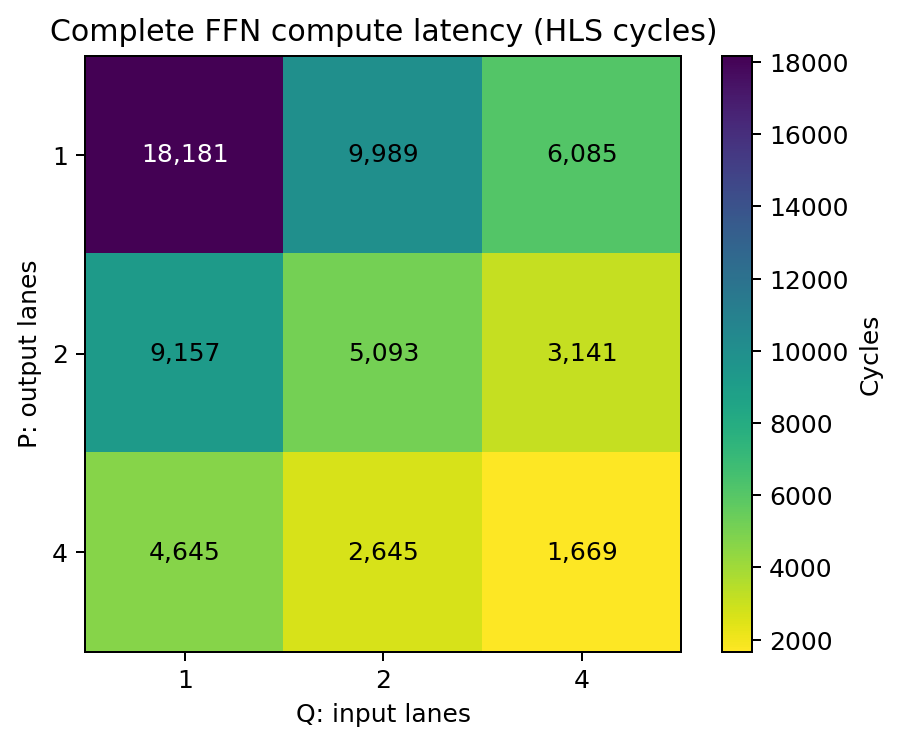
\includegraphics[width=0.88\linewidth]{banked_latency.png}
 \caption{Computation-cycle estimates across the nine pipelined banked designs.
 Both dimensions of parallelism matter; equal $PQ$ does not imply equal latency.}
 \label{fig:banked}
\end{figure}

\subsection{Insufficient memory ports}
U44 allocates 32 DSPs, matching B44 and K44, but its main loops achieve II=16
rather than the requested II=1. HLS reports memory-port scheduling limitations
(\code{HLS 200-885}) for this design. With sixteen scalar weight accesses
requested per input-group iteration and a single read port per layer, the
operand demand cannot be served in one cycle. U44 consequently requires 17,029
computation cycles, only $1.07\times$ faster than B11 despite using sixteen
times as many DSPs. B44's matched banking reduces this to 1,669 cycles, a
$10.20\times$ reduction relative to U44. The achieved II, scheduling diagnostics,
and latency comparison together support a memory-bandwidth explanation.

\subsection{Packed words and BRAM utilization}
K44 matches B44's 1,669-cycle estimate and II=1 while reducing total estimated
BRAM usage from 36 to 20 units, or 44.4\%. Weight memories alone decrease from
32 to 16 BRAM\_18K units; four additional units belong to the HLS memory
interface. The B44 organization creates sixteen scalar banks per layer, each
containing 512 sixteen-bit weights. K44 creates four banks per layer, each
containing 512 sixty-four-bit words. Both provide the same sixteen weights per
input-group iteration, but packing makes better use of physical memory capacity
in this synthesis result. K44 also reduces LUTs from 12,653 to 11,665 and FFs
from 16,328 to 16,034 compared with B44. This is a measured result for this
shape, precision, storage constraint, and tool version, not a claim that packing
always dominates banking.

\begin{figure}[tb]
 \centering
 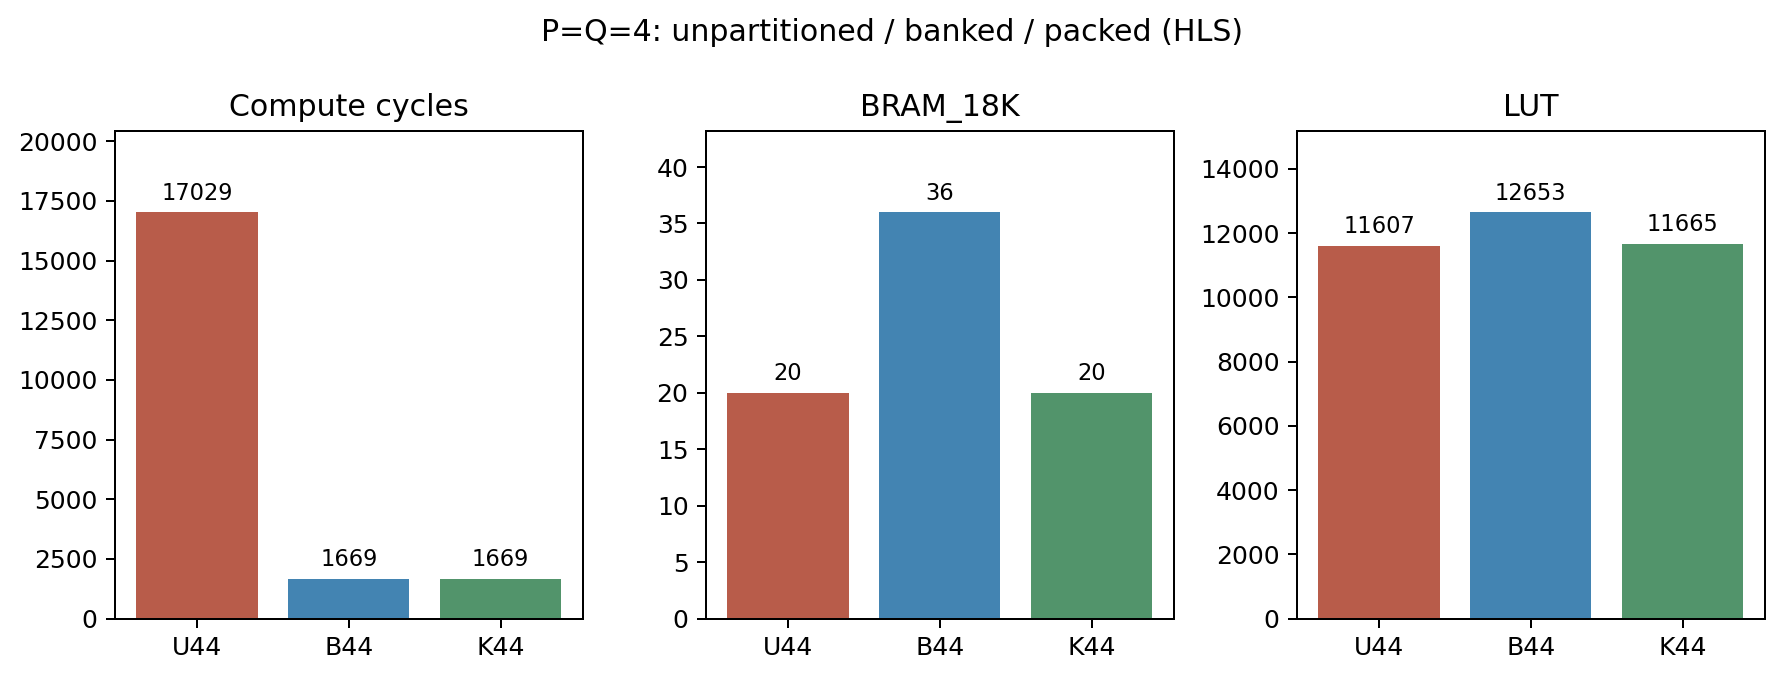
\includegraphics[width=0.92\linewidth]{memory_comparison.png}
 \caption{Comparison of the unpartitioned, banked, and packed designs at
 $P=Q=4$. Compute parallelism alone does not determine effective throughput
 or physical memory cost. Values are HLS estimates.}
 \label{fig:memory}
\end{figure}

\subsection{RTL latency and parameter loading}
Table~\ref{tab:rtl} reports actual top-level operation cycles from the successful
co-simulations. The measured RUN values are constant across the eight inference
calls in each suite. B11/K44 gives a $10.86\times$ RTL RUN ratio, consistent with
the HLS comparison, but these values include the co-simulation memory model and
use a different measurement boundary from \code{ffn_compute}. The small
numerical differences between the HLS and RTL cycle columns should therefore
not be interpreted as measurement error or combined into a single latency
series.

\begin{table}[tb]
\centering
\caption{Top-level RTL co-simulation cycles under the tool's AXI memory model.
Each design has four LOAD and eight RUN measurements; the minima and maxima
are equal within each operation type. These are not board timings.}
\label{tab:rtl}
\begin{tabular}{lrr}
\toprule
Design & RUN cycles & LOAD cycles\\
\midrule
B11 & 17,869 & 29,152\\
B44 & 1,645 & 29,152\\
U44 & 17,005 & 29,152\\
K44 & 1,645 & 12,768\\
\bottomrule
\end{tabular}
\end{table}

Parameter transfer size is identical across designs, but conversion into the
on-chip layout has a different schedule. K44 loads parameters in 12,768 cycles,
compared with 29,152 for the scalar-word organizations. This cost is reported
separately because repeated RUN calls reuse weights. The intended inference
comparison does not reload 33,152 bytes for every 128-byte input.

\subsection{Implementation of the selected candidates}
K44 is selected as the optimized deployment candidate because it ties the
lowest HLS latency while requiring less BRAM and logic than B44. B11 and K44
both complete placement and routing at the common 100\,MHz target.
Table~\ref{tab:impl} uses full implemented-design reports, including the
integration logic; its counts are distinct from the HLS estimates.

\begin{table}[tb]
\centering
\small
\caption{Full implemented-design resources and timing at 100\,MHz.
BRAM tiles are 36\,Kb equivalents; nine tiles equal eighteen BRAM\_18K units.
WNS is worst setup slack and WHS is worst hold slack.}
\label{tab:impl}
\begin{tabular}{lrrrrrr}
\toprule
Design & LUT & FF & DSP & BRAM tiles & WNS (ns) & WHS (ns)\\
\midrule
B11 & 8,931 & 16,046 & 2 & 9 & 0.387 & 0.024\\
K44 & 10,264 & 18,169 & 32 & 9 & 0.350 & 0.016\\
\bottomrule
\end{tabular}
\end{table}

The implemented K44 design retains the same BRAM-tile count as B11 while using
32 rather than two DSPs, 14.9\% more LUTs, and 13.2\% more FFs. Positive setup
and hold slack show that both designs meet
the implemented constraint. They do not establish a higher maximum operating
frequency, validate the host driver on hardware, or determine end-to-end speedup.

\section{Deployment Verification and Board Evaluation}
\subsection{Completed local integration checks}
The deployment review specifically addresses reset and control-path failures
that can make a processor's first PL register access stop responding. The reset
controller's auxiliary input is active-low and must be tied high when unused.
Tests using the vendor-generated reset netlist reproduce the nonresponding
control interface under the erroneous tie-low condition and verify reset release
and a completed control read with the implemented tie-high connection.

For both B11 and K44, additional tests exercise the actual HLS control RTL:
64-bit pointer halves, byte write strobes, operation selection, repeated start
and completion, clear-on-read completion status, delayed AXI address/data
phases, response backpressure, and reset recovery. A separate test connects the
complete generated FFN RTL to that reset controller and a bounded, stalling AXI
memory model. It checks invalid and unloaded operations without DDR access,
LOAD, two successive inferences, reset, rejection of stale parameters, a new
LOAD, and another inference. All outputs match the independent reference;
reads and writes remain within the modeled parameter, input, and output
allocations. Each design transfers 8,336 read words and 48 write words during
this additional suite. These tests do not include PS7, SmartConnect behavior,
Linux, or CPU caches.

The host is organized into explicit preflight, programming, first control
access, allocation, correctness, and timing stages. Package hashes bind the
bitstream, HWH, host files, fixtures, and verification evidence. Metadata checks
reject fourteen injected wiring/configuration faults for each candidate,
including permanently asserted reset, wrong clock, wrong AXI connection, and
wrong register or memory address. These checks remain enabled under Python
optimization. Twenty host regression tests check timeout/interruption handling, register
failures before and after launch, non-idle and auto-restart states, and session
ownership. An uncertain transaction blocks further launches and buffer release;
a persistent marker prevents a new notebook session from silently bypassing
that state. A Python polling timeout cannot recover a stalled MMIO transaction,
so these controls reduce known risks rather than guarantee absence of a physical
board hang.

\subsection{Board protocol and integration findings}
The board experiment used the reserved course PYNQ-Z2 \code{pynq2} on
November 18, 2026. The image runs PYNQ 2.5, Python 3.6.5, NumPy 1.13.3, and
Linux 4.19.0. The PL clock was verified as 100\,MHz and the CPU clock read as
650\,MHz. The C++ reference was compiled on the board with GCC 7.3.0 using
\code{-std=c++17 -O3}. The image did not expose CPU-frequency governor files;
we did not change CPU frequency, affinity, or operating-system scheduling.

Two host issues were found and corrected during integration. The image's older
NumPy requires filename strings for \code{fromfile}, so explicit string
conversion was added. A second issue involved the HLS control handshake:
\code{ap_done} and \code{ap_idle} are independently registered and need not be
visible in the same control read. The earlier host stopped when it observed
\code{0x0a} (done and ready, without idle). Diagnostic reads then returned idle,
the status was successful, and every output of that completed inference matched
the reference. The session was retired after that positive completion check.
The corrected host remembers the clear-on-read done flag and continues polling
until idle is also observed, under the original timeout. New control-RTL and
host regressions cover completion before idle and timeout if idle never arrives.
No hardware bitstream changes were required. Both candidates were rerun from
fresh sessions with the same corrected \code{audit3} host; earlier attempts are
retained but excluded from the final comparison.

Each final candidate passed an initial guard check, a known-input smoke test,
and all 206 inferences across nine parameter sets. Benchmarking then performed
20 warm-ups and three rounds of 1,000 calls; every measured output matched.
The CPU reference independently validated both layers for 206 cases and used
the same 3,000-call workload. Sessions closed normally, buffers were released,
and their kernels were stopped. The board remained in the operating state;
there was no board hang or reboot during the experiment.

The FPGA host interval includes input-buffer copy and cache flush, control
register writes, polling until completion and idle, return status, and output
invalidation and copy. It excludes programming, parameter LOAD, input shape/type
checks, result comparison, and file I/O. CPU timing measures compiled computation
on resident arrays, excluding file I/O and validation. These measurements compare
the implemented application paths; they do not isolate FPGA and CPU arithmetic
at identical software boundaries. Build-host CPU smoke measurements are not
included.

\subsection{Measured latency}
Table~\ref{tab:board} reports the final \code{audit3} measurements. K44 reduces
median host latency from 1,103.991 to 964.715\,$\mu$s, giving a
$1.14\times$ speedup and a 12.6\% latency reduction. This is much
smaller than the $10.89\times$ HLS computation ratio. The CPU results following
the two FPGA tests agree closely, at 143.499 and 142.971\,$\mu$s.
The tested K44 host path therefore takes $6.75\times$ the time of its
corresponding compiled CPU computation. The present Python/FPGA interface does
not outperform the board CPU for one input at a time.

\begin{table}[tb]
\centering
\small
\caption{Physical board2 measurements in microseconds. Each row contains 3,000
correct calls (three rounds of 1,000). FPGA rows include the Python host path;
CPU rows measure compiled computation. Maxima are retained, not trimmed.}
\label{tab:board}
\begin{tabular}{lrrr}
\toprule
Execution path & Median ($\mu$s) & P95 ($\mu$s) & Maximum ($\mu$s)\\
\midrule
B11: Python/FPGA host & 1,103.991 & 1,157.015 & 1,504.677 \\
K44: Python/FPGA host & 964.715 & 1,061.408 & 10,314.825 \\
C++ CPU after B11 & 143.499 & 146.283 & 203.455 \\
C++ CPU after K44 & 142.971 & 144.789 & 386.800 \\
\bottomrule
\end{tabular}
\end{table}

The per-round FPGA medians are 1,103.417, 1,102.705, 1,105.723\,$\mu$s for B11 and
964.669, 968.777, 962.769\,$\mu$s for K44. K44 also exhibits a 10.315\,ms maximum sample.
All samples are retained. This experiment does not isolate the cause of that
outlier; scheduling and other system effects remain possible, so the maximum
must not be interpreted as a hardware execution bound. The observation supports
using medians and percentiles while preserving raw samples, rather than claiming
deterministic end-to-end latency from one board session.

LOAD timing was saved separately. The individual LOAD observations are not a
controlled repeated loading benchmark, and their variability does not support a
board-level loading-speedup claim. The primary inference comparison consistently
keeps weights resident on chip.

\subsection{Where the host time is spent}
A separate diagnostic run adds timestamps around input-buffer preparation,
control and execution, and output-buffer retrieval. It uses 100 extra verified
calls per design; these samples are not substituted into the primary benchmark.
For B11, the phase medians are approximately 214.7, 616.8, and
329.6\,$\mu$s. For K44 they are 213.7, 475.5, and 328.8\,$\mu$s.
Thus input and output buffer work alone totals approximately 542.5\,$\mu$s
for K44, already more than its corresponding CPU computation time. The
control/execution phase includes register access, polling, and actual accelerator
and memory-system work; it is not a direct measurement of hardware kernel time.

\begin{figure}[tb]
 \centering
 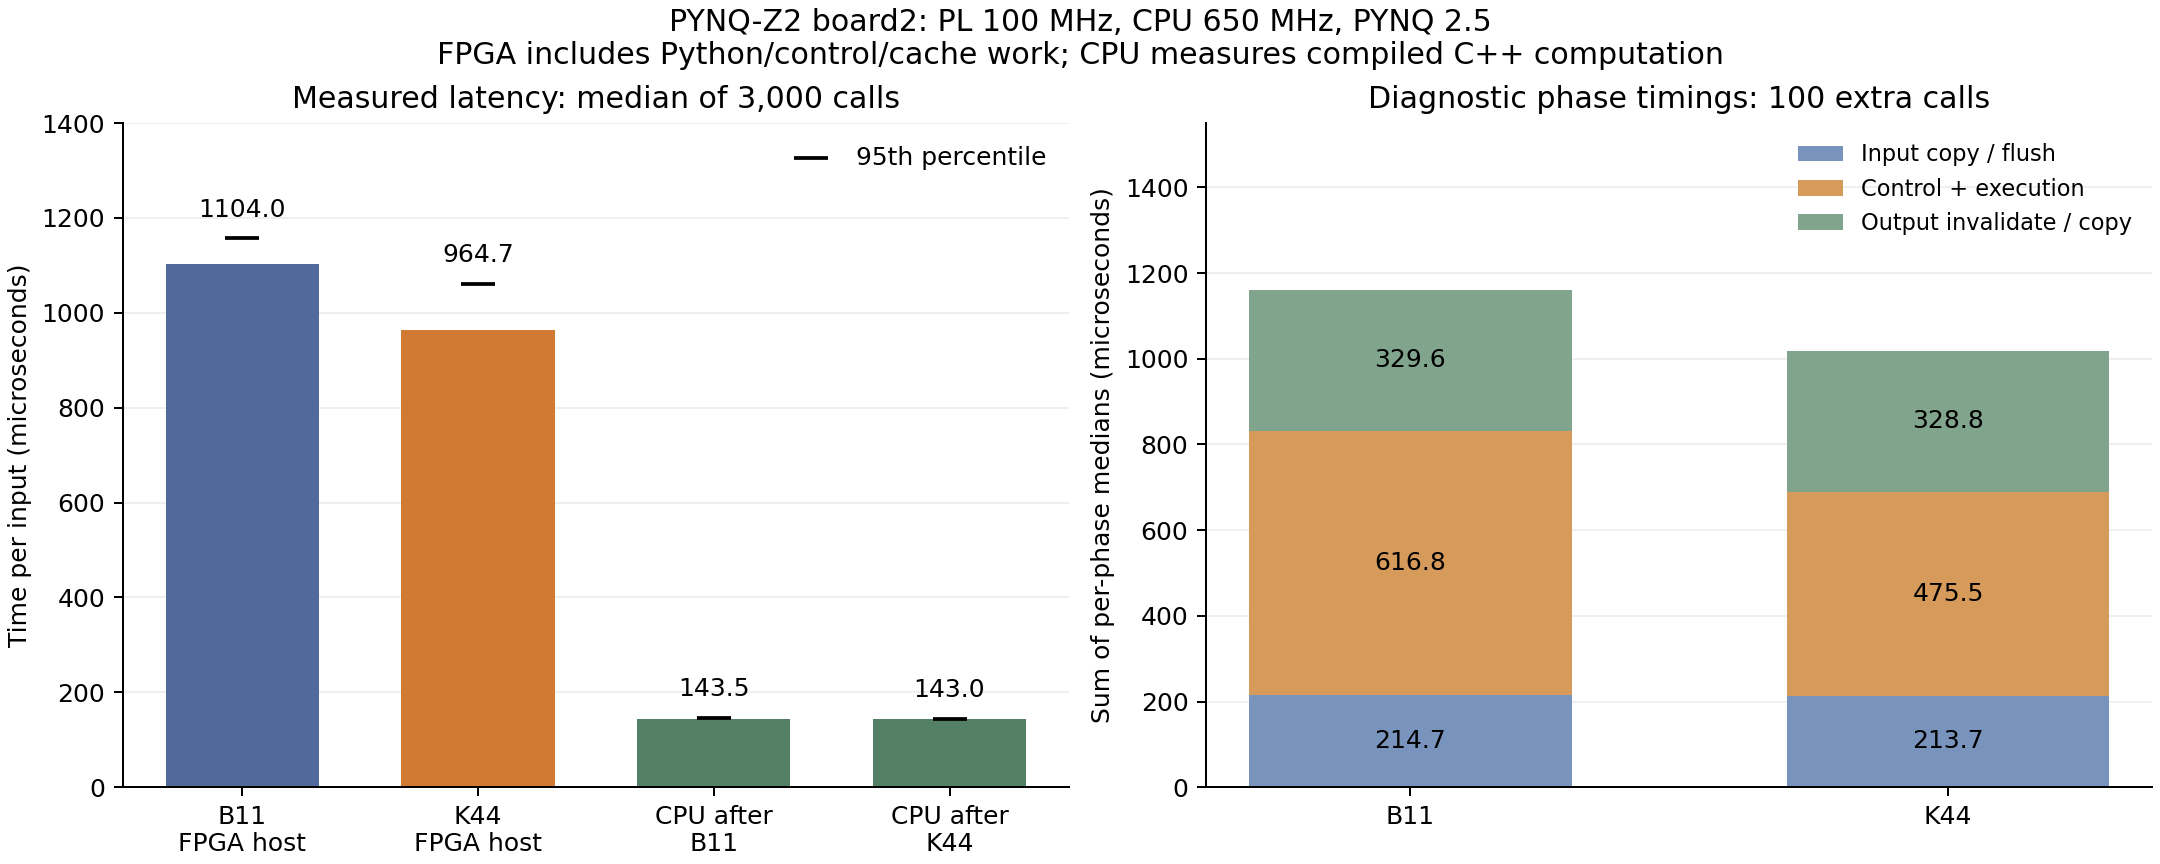
\includegraphics[width=\linewidth]{board_latency.png}
 \caption{Measured host and CPU latency (left), and separate diagnostic phase
 timings (right). The right panel stacks per-phase medians from 100 calls with
 additional timestamps; its totals need not equal the primary benchmark medians.
 Both candidates use the same final host revision.}
 \label{fig:board}
\end{figure}

\section{Discussion and Limitations}
The three architectural questions have distinct answers. Increasing parallelism
reduces complete computation latency, but equal lane counts can have different
overheads. Matching weight ports to lane demand is necessary to sustain II=1.
Finally, packing adjacent weights preserves operand bandwidth with fewer BRAMs
than scalar banking for the measured $4\times4$ configuration. Together, the
U44/B44/K44 comparison identifies a memory-organization effect while holding
the requested arithmetic parallelism constant.

The diagnostic results explain why faster matrix--vector computation produces
only a modest end-to-end gain for this small workload. Further system-level
optimization should target buffer synchronization and host control costs before
adding arithmetic lanes. A compiled host path, fewer redundant control writes,
or a different submission interface are possible future experiments; no benefit
from those unimplemented alternatives is claimed here. Batching would change the
single-input workload and must be evaluated separately if introduced.

These results come from one physical board and one reservation, with three
measurement rounds and the standard running PYNQ image. They establish functional
operation and the observed application-path comparison, not reliability across
all boards, maximum frequency, power efficiency, or a hardware-only speedup.
No on-board cycle counter was added, so simulation cycles remain explicitly
separate from measured host latency.

\section{Conclusion}
The local experiments show that useful unrolling depends on matching weight
bandwidth to arithmetic demand. The unpartitioned $4\times4$ design consumes
32 DSPs yet provides little latency improvement over the pipelined scalar
baseline; cyclic banking restores II=1. Packing adjacent weights preserves that
latency while reducing HLS-estimated BRAM consumption by 44.4\% relative to
scalar banking. B11 and K44 both meet the 100\,MHz implementation constraint and
pass functional, RTL, reset, control, and physical-board validation. The
$10.89\times$ HLS compute improvement translates to a measured $1.14\times$
Python/FPGA host improvement; this path remains slower than the compiled board
CPU. The project therefore demonstrates both the value of matching on-chip
memory bandwidth to unrolling and the importance of host/interface cost when
translating that gain to a complete single-input accelerator.

\appendix
\section{Evidence and Reproducibility}
Source code, report source, final deployment packages, and measurement evidence
are available at
\href{https://github.com/aliothren/ECE506_Project}{github.com/aliothren/ECE506\_Project}.
The numerical and parameter
contracts are in \code{spec.md}; configurations are in \code{experiments.csv}.
The table sources are \code{results/hls_results.csv} and
\code{results/implementation_results.csv}. Figures use the existing PNG files
under \code{figures/}. Selected unmodified HLS, co-simulation, and implementation
reports are preserved under \code{results/hls_reports/}, with a SHA-256 manifest
mapping them to their original run paths. The full vendor build directories and
earlier failed attempts remain in local archival storage and are omitted from
Git. The deployment archives include the control/reset testbench sources,
verification records, and simulation logs tied to each released bit/HWH pair.

The final deployment archives have the suffix \code{_audit3.zip}. Their
immutable build manifests retain the original \code{board_tested=false} field;
post-build board validation is recorded separately in
\code{results/board_results.json}, bound to each uploaded ZIP and bit/HWH hash.
Raw CSVs, environment data, completed notebooks, stage logs, and normal-close
records are retained under \code{results/board2_20261118/B11} and
\code{results/board2_20261118/K44}. Earlier software-integration attempts are in
local archival directories and are not included in the final comparison. The
collection script checks all sample indices, correctness flags, medians,
percentiles, manifest identities, and release hashes. The board figure is
reproducible from those records. Operational instructions are documented
separately in \code{board/README.md}.

A fresh clone can validate fixture regeneration, the C++ reference, host
regressions, published report hashes and tables, board raw samples, and release
contents without a board or vendor tools; commands are in
\code{docs/reproduce.md}. Rebuilding HLS and the overlays requires Vitis
HLS/Vivado 2025.1. Repeating physical measurements requires a separately
authorized PYNQ-Z2 session. This delivery contains TeX and PNG source assets;
no report PDF was generated, and TeX checks were structural rather than a
typesetting-engine run.

\begin{thebibliography}{9}
\bibitem{cilardo2015}
A. Cilardo and L. Gallo, ``Interplay of loop unrolling and multidimensional
memory partitioning in HLS,'' in \emph{Design, Automation \& Test in Europe
Conference \& Exhibition (DATE)}, pp. 163--168, 2015.
\href{https://past.date-conference.com/proceedings-archive/2015/pdf/0798.pdf}{Full text}.

\bibitem{blott2018}
M. Blott, T. Preusser, N. Fraser, G. Gambardella, K. O'Brien, and Y. Umuroglu,
``FINN-R: An End-to-End Deep-Learning Framework for Fast Exploration of
Quantized Neural Networks,'' \emph{ACM Transactions on Reconfigurable Technology
and Systems}, vol. 11, no. 3, 2018.
\href{https://doi.org/10.1145/3242897}{doi:10.1145/3242897};
\href{https://arxiv.org/abs/1809.04570}{author preprint}.
\end{thebibliography}
\end{document}
